\documentclass[aspectratio=169]{beamer} % 使用 16:9 宽屏

% 引入必要的宏包
\usepackage[UTF8]{ctex}
\usepackage{amsmath}
\usepackage{amssymb} 
\usepackage{bm}
\usepackage{graphicx}
\usepackage{booktabs}
\usepackage{tcolorbox}
\usepackage{tikz} 
\usepackage{pifont} 

% 主题与颜色设置
\usetheme{Madrid} 
\usecolortheme{default}
\setbeamertemplate{navigation symbols}{} 
\setbeamertemplate{footline}[frame number] 

% 自定义高亮颜色
\definecolor{myblue}{RGB}{33, 113, 181}
\definecolor{myred}{RGB}{203, 24, 29}
\definecolor{mygreen}{RGB}{44, 160, 44}

\title[Distribution Leakage in Cross-Silo FL]{On Data Distribution Leakage in Cross-Silo Federated Learning}
\subtitle{2024 TKDE —— 跨孤岛联邦学习中的分布推断攻击}
\author{文献分享}
\date{\today}

\begin{document}

\begin{frame}
    \titlepage
\end{frame}

\begin{frame}{Agenda}
    \tableofcontents[hideallsubsections]
\end{frame}

% ==========================================
\section{1. 前置知识 (Preliminaries)}
% ==========================================

\begin{frame}{1.1 跨孤岛联邦学习 (Cross-Silo FL)}
    \begin{itemize}
        \item \textbf{定义：} 多个机构（如银行、医院）在不交换原始数据的情况下，协作训练一个共享模型。
        \item \textbf{交互流程：} 
        \begin{enumerate}
            \item \textbf{本地训练：} 客户端利用本地数据计算梯度 $\nabla L(x, y; \theta)$。
            \item \textbf{参数同步：} 客户端上传模型更新（梯度或权重差）至中心服务器。
            \item \textbf{全局聚合：} 服务器执行 FedAvg（如权重平均）更新全局模型。
        \end{enumerate}
        \item \textbf{核心特征：} 参与方数量少（Silo）、计算能力强、数据量大。
    \end{itemize}
\end{frame}

\begin{frame}{1.2 差分隐私 (Differential Privacy) 在 FL 中的应用}
    为了防止梯度泄露个体隐私，通常引入 \textbf{DP-SGD} 防御机制：
    
    \begin{tcolorbox}[colback=blue!5,colframe=myblue,title=DP-SGD 核心步骤]
        \begin{enumerate}
            \item \textbf{裁剪 (Clipping)：} 限制每个梯度向量的 $\ell_2$ 范数，防止单个极端样本主导更新。
            \item \textbf{加噪 (Noise Addition)：} 在聚合梯度中注入高斯噪音 $n \sim \mathcal{N}(0, \sigma^2 C^2)$。
        \end{enumerate}
    \end{tcolorbox}
    
    \textbf{隐私承诺：} 攻击者无法以显著概率判断训练集中是否包含“张三”这一条特定记录。
\end{frame}

% ==========================================
\section{2. 问题陈述与威胁模型 (Problem Statement)}
% ==========================================

\begin{frame}{2.1 什么是分布泄露？ (Problem Definition)}
    \begin{columns}
        \begin{column}{0.45\textwidth}
            \textbf{攻击者的目标：} \\
            推断出参与方 $k$ 的\textbf{全局统计分布}，包括：
            \begin{itemize}
                \item \textbf{特征分布 $P(X)$：} 数据在各特征维度上的均值、方差。
                \item \textbf{标签分布 $P(Y)$：} 训练集中正负样本的真实比例（极具商业价值）。
            \end{itemize}
            \vspace{0.2cm}
            \textbf{为什么是盲区？} \\
            DP 保护了个体，但为了保证模型可用性，它必须保留数据的统计特性。
        \end{column}
        \begin{column}{0.55\textwidth}
            \begin{center}
                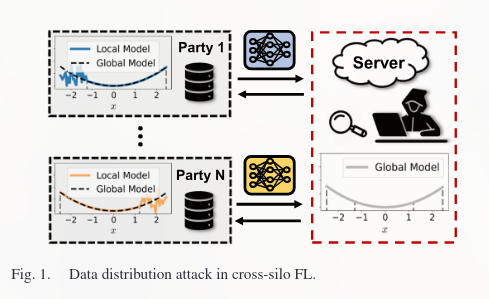
\includegraphics[width=\textwidth]{fig_fl_threat.png}
            \end{center}
        \end{column}
    \end{columns}
\end{frame}

\begin{frame}{2.2 诚实但好奇的服务器 (Threat Model)}
    \begin{itemize}
        \item \textbf{服务器能力：} 
        \begin{itemize}
            \item 观察每一轮客户端上传的梯度更新。
            \item 知道当前的全局模型参数 $\theta_t$。
            \item \textbf{无先验知识：} 攻击者没有参与方的辅助数据（无影子数据）。
        \end{itemize}
        \item \textbf{防御假设：} 客户端可能开启了裁剪和加噪形式的差分隐私防御。
    \end{itemize}
\end{frame}

% ==========================================
\section{3. 分布推断攻击方案 (Attack Methodology)}
% ==========================================

\begin{frame}{3.1 攻击分类：根据模型性质因地制宜}
    \begin{tcolorbox}[colback=white,colframe=mygreen,title=两套推断机制]
    \begin{itemize}
        \item \textbf{方案 A：针对可微分模型 (如神经网络)}
        \begin{itemize}
            \item 利用梯度作为优化约束，提出 \textbf{PGDA (梯度分布攻击)}。
            \item 核心思想：寻找一组虚拟分布，使其产生的梯度与观测梯度最匹配。
        \end{itemize}
        \item \textbf{方案 B：针对不可微分模型 (如决策树、逻辑回归)}
        \begin{itemize}
            \item 无法通过梯度求导，攻击者通过分析参数更新的数值特征，建立统计关联进行推断。
        \end{itemize}
    \end{itemize}
    \end{tcolorbox}
\end{frame}

\begin{frame}{3.2 PGDA 工作流：如何从梯度逆推分布？}
    \begin{columns}
        \begin{column}{0.45\textwidth}
            \textbf{PGDA (Property/Prior Gradient Distribution Attack)：}
            \begin{enumerate}
                \item \textbf{特征重构优化：} 初始化虚拟输入数据分布。
                \item \textbf{梯度匹配损失：} 计算虚拟数据产生的梯度与截获梯度的距离。
                \item \textbf{反向传播更新：} 不断调整虚拟数据的分布参数，使 Loss 极小化。
            \end{enumerate}
        \end{column}
        \begin{column}{0.55\textwidth}
            \begin{center}
                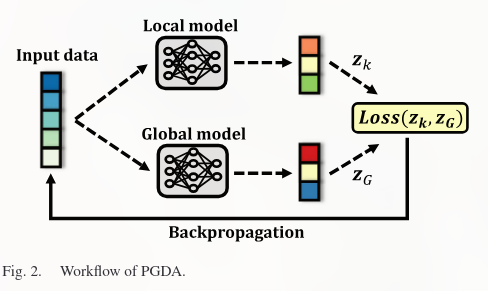
\includegraphics[width=\textwidth]{fig_pgda.png}
            \end{center}
        \end{column}
    \end{columns}
\end{frame}

\begin{frame}{3.3 PGDA 核心：基于梯度匹配的数学优化}
    攻击者求解以下优化问题来逼近真实分布：
    \begin{equation}
        \min_{\mathbf{D}_{dummy}} \mathcal{L}_{match} = \left\| \nabla W(\mathbf{D}_{dummy}, \theta) - \nabla W_{intercepted} \right\|^2 + \alpha \cdot \mathcal{R}(\mathbf{D}_{dummy})
    \end{equation}
    
    \begin{itemize}
        \item $\nabla W_{intercepted}$：截获的真实梯度更新。
        \item $\mathbf{D}_{dummy}$：攻击者构造的虚拟数据分布参数。
        \item $\mathcal{R}(\cdot)$：正则化项，用于确保生成分布的合理性。
    \end{itemize}
    
    \textbf{关键洞察：} 该优化过程不涉及具体样本还原，只关注分布级别的参数。
\end{frame}

% ==========================================
\section{4. 实验评估与防御分析 (Evaluation \& Defense)}
% ==========================================

\begin{frame}{4.1 击穿最强防御：为什么 DP 失效了？}
    \begin{columns}
        \begin{column}{0.45\textwidth}
            \textbf{实验观察：}
            \begin{itemize}
                \item \textbf{个体的干扰：} 噪音很大时，单个样本的特征被完全模糊。
                \item \textbf{总体的抗噪性：} “分布”是成千上万个样本的平均统计特性。
                \item \textbf{结论：} 零均值的高斯噪音在聚合过程中会相互抵消，宏观分布特征对 DP 噪音具有天然的鲁棒性。
            \end{itemize}
        \end{column}
        \begin{column}{0.55\textwidth}
            \begin{center}
                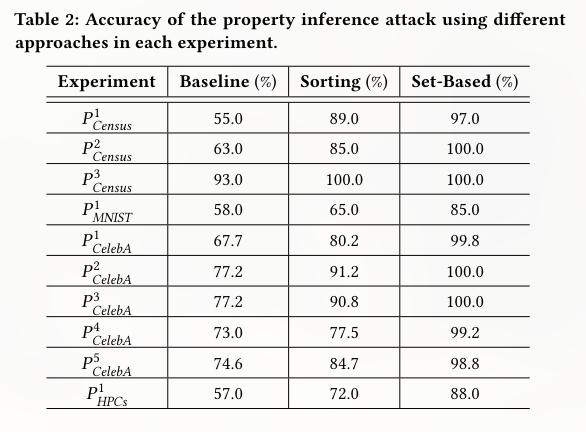
\includegraphics[width=\textwidth]{fig:result.png}
            \end{center}
        \end{column}
    \end{columns}
\end{frame}

% ==========================================
\section{5. 总结与启示 (Conclusion)}
% ==========================================

\begin{frame}{5.1 研究启示}
    \begin{tcolorbox}[colback=blue!5,colframe=myblue,title=核心结论 (Takeaways)]
        \begin{itemize}
            \item \textbf{隐私保护的错位：} 跨孤岛场景下，“宏观分布”往往比“微观记录”更具商业敏感性，但现有防御却无能为力。
            \item \textbf{PGDA 的威力：} 首次证明了无需任何辅助数据，服务器就能以极高精度还原本地数据分布。
        \end{itemize}
    \end{tcolorbox}
\end{frame}

\begin{frame}
    \begin{center}
        \Huge \textbf{Q \& A} \\
        \vspace{1cm}
        \Large 感谢聆听！
    \end{center}
\end{frame}

\end{document}